\documentclass{scrartcl}

\usepackage[en,break]{ukon-infie}
\usepackage{hyperref}
\usepackage{bookmark}
\Names{L. Kr\"amer}
\Term{SS 13}
\Lecture[SWP]{Softwareprojekt}
\date{10.05.2013}
\title{Protokoll 1. Treffen Freitag 26.04. 13:00}
\def\oder{\vee}
\def\und{\wedge}
\bookmarksetup{
  numbered,
  open
}
\renewcommand*{\thesection}{\arabic{section}}

\begin{document}
\maketitle
%\tableofcontents
\section{Ort}
Unterhalb der Mensa, 15:30-17:30
\section{Anwesenheit}
Philipp Hilpert, Matthias Kraus, Rebecca Kehlbeck, Fabian Vollmer, Nicolas Siebeck, Matthias Miller \\
\textbf{Entschuldigt:} Leonard Krämer
\vspace*{-0.5cm}
\section{Agenda}
\begin{itemize}
\item Letztes Treffen
\item Agenda bearbeiten
\item Tasks
\item Ausblick
\item Ideen Fragen und sonstige TO DO's
\end{itemize}
\vspace*{-0.5cm}
\section{Tasks}
Ausgearbeitete Agenda bearbeiten (siehe Anhang) \\
Projektplan mit Latex erstellen \\
Kontaktdokument in Googledocs ausfüllen\\
\vspace*{-0.5cm}
\section{Ausblick}
Milestones im Projektplan \\
Projektplan fertig machen und einreichen. \\
Projektplanpräsentation nächste Woche. \\
Concall mir Herrn de Ridder. \\
Nach den Requirements gleich das SRS anfangen. \\
Treffen bei den Projektplanpräsentationen.
\vspace*{-0.5cm}
\section{Ideen Fragen und sonstige TO DO's}
N/A
\vspace*{-0.5cm}
\section{Anhang}
\setcounter{section}{0}
\renewcommand*{\theHsection}{chX.\the\value{section}}
\emph{Was herauskam immer kursiv. Agenda:}
\section{Begrüßung}
%Hallo, bla wie war eure Woche?, wer macht Protokoll? Vorstellen was wir heute machen; Inhaltsverzeichnis stellt das da.
\section{Letzte Woche}
Jeder trägt kurz vor, was er seit dem letzten Treffen gemacht hat, thematisch zusammengefasst. 
\\ Google Group erklären, Google Drive erklären. Haben alle Zugriff? Wenn nein nach dem Treffen lösen, sollte es ein Gruppenproblem sein gleich machen.
 \\ \emph{check, wird benutzt, forumartig, damit eine Knoledgebase entsteht}
\\ Wenn möglich kleine Präsentation über die Funktionen von Git und wie man es installiert/benutzt. \\
\emph{Rebecca übernimmt den Task}
 \\ Agreedo \\
 \emph{Agreedo wird als Plattform für die Agenda benutzt}
 \\	Bibliotheken erklären, Fabian, Matthias, Matthias \\ 
 Wichtige Punkte dabei: 
	 \begin{itemize}
 	\item Schnittstellen
 	\item Funktionen der Bibliotheken
	 \item Welche Interfaces werden zur Verfügung gestellt
	 \end{itemize}
	 \emph{Sie sind unsere 'Library Experts'}
\section{Rückfragen}
Welche Fragen haben sich beim Bearbeiten der Tasks ergeben? Welche Empfehlungen habt ihr an die anderen? \\ \emph{N/A}
\section{Personenbezogenes}
Nochmal wer hat wann keine Zeit? Doodle für einen regelmäßigen Termin machen, wöchentliches Treffen wäre optimal, Herr de Ridder will da afaik dabei sein(?). \emph{Will er nicht}
\\ Wann hat wer keine Zeit? Ich bin über das Wochenende 21.06. nicht da, hab eine Klausur am Ende des Semesters. \\ \emph{Eigentlich haben alle immer Zeit, man fährt öfters übers Wochenende heim}
\section{jobs}
\begin{itemize}
\item \textbf{Projektmanager} - Leonard - Sorgt dafür, dass alle aufgaben innerhalb des Zeitplanes gemacht wird. Risikoabschätzung. Änderungsmanagement.
\item \textbf{Versions-(Datei-)Manager} - Rebecca - Sorgt dafür, dass die Daten sicher gespeichert sind und in der richtigen Version vorliegen. Struktur der Daten festlegen. Sorge tragen, dass die Struktur eingehalten wird (nicht alles selbst organisieren, sondern Leute auf Fehler hinweisen und Lösung erarbeiten)
\item \textbf{Dokumentenmanager} - frei (Matthias Miller?) - Sorgt für einheitliche, lückenlose Dokumentation. \textbf{Wichtig, da davon die Note abhängt!!!} (Die Aufgabe ist nicht die Dokumentation alleine zu erstellen, sondern Format festlegen und Leute dazu antreiben die Doku zu erstellen)
\item \textbf{Spezifikationsmanager} - frei- Experte für Requirements \\ Verantwortlich für Requirements und Änderungen \\ SDD / SRS prüfen, verantwortlich für die Erstellung dieser \\ Sicherstellen, dass die Spezifikationen eingehalten werden.
\item \textbf{Testmanager} - frei - Experte für Testing. \\ Sicherstellen, dass alles mindestens ein mal getestet wurde. Enge Zusammenarbeit mit Spezifikationsmanager. Festlegen wie getestet wird, Tests überprüfen.
\item \textbf{Software support} 'The expert on development tools. Installs (or helps in-
stalling) them and provides knowledge on their proper usage to the other
team members.'
\item \textbf{Library expert} Knows how to use a particular library and its strengths and
weaknesses. \textbf{SWING, ISGCI, JgraphX}
\item Weitere Jobs? Möglich: Experten für  Design, Codereview... (ich weiß nicht in wie weit diese Jobs essenziell sind oder ob es Sinn ergibt sie speziell zuzuweisen, da wir alle das wissen haben sollten. Eine Zuweisung ergibt insofern Sinn, dass dann nicht alle in die Tiefe müssen und man einen Ansprechpartner hat.)
\end{itemize}
\emph{- Jobs \begin{itemize}
\item Leo: Projektmanager
\item Becci: Verwaltung
\item Kraus: Spezifikationsmanager
\item Fabi: Testmanager
\item Miller: Dokumentmanager
\item Philipp: stellvertretender Projektmanager und nach bedarf Verwaltung, Testmanager
\item Nico: Präsentationen und Protokolle
\end{itemize}}

\section{Requirements Sammeln}
\textbf{Hier beginnt der Hauptteil des Meetings}
Alle sollten welche herausgearbeitet haben, wenn nicht dann gemeinsam erarbeiten,
PDF liegt auf Google Drive. Man kann es auch auf der Seite http://www.informatik.uni-konstanz.de/ag-ernst-de-ridder/lehre/ erreichen, wenn man sich anmeldet.
Funktionale und nicht funktionale Anforderungen. Siehe Seng Folien!!
\\ \emph{Dieser Teil ging wirklich lange}
%hier füge ich welche ein

\section{Ideen Sammeln, was man machen kann}
\begin{description}
\item Alle Ideen sind gut und werden ohne Kritik aufgenommen und diskutiert.
\item Was wären wünschenswerte Features \\ Zooming, möglichst wenige Überschneidungen von Kanten, Interaktivität (Super- oder Subknoten ein-/ausblenden, Knoten färben...
\item Was kann das Framework? \\ Wichtig um zu den Zeitaufwand zu bewerten.
\item Dabei Machbarkeit im Kopf behalten. \\
\emph{Auf Papier, daraus resultierte der Projektplan s.u.}
\end{description}
\section{Wie}
Wie können die Spezifikationen und Features umgesetzt werden? Wie viel Zeit wird (geschätzt) gebraucht. Entweder Stunden/ Wochen als Einheit oder loc (Lines of code). \\
\emph{Auf Papier, daraus resultierte der Projektplan s.u.}
\section{Zeitplan Skizzieren}
Als Prozessmodell schlage ich vor Rapid Prototyping mit dem Wasserfallmodell zu verbinden, Dadurch stellen wir eine gute Dokumentation sicher und minimieren dabei das Risiko.
Überlegt welche Tasks man parallel ausführen kann, was nach was kommen muss. Ordnet alles auf einer Timeline an. Möglichst alle 1-2 Wochen einen Milestone einführen. Feinkörnige Planung für die ersten 1-2 Wochen, dann grob.
Feste Termine: \begin{itemize}
\item Dienstag 30.4. Zeitplan steht fest
\item Dienstag (frühestens)\textbf{ 30.4.} - (spätestens) 7.5. SRS erste Revision ist fertig
\item Iterationen mit Mockups um festzustellen, wie das graphische Frontend aussehen soll. Wenn der erste Prptotyp alles erfüllt Requirements prüfen und SDD schreiben.
\item Dienstag 14.5. - 21.4. SDD, erste Revision ist fertig
\item Dienstag 2.7. Akzeptanztest und Deployment im Erfolgsfall
\end{itemize}
Klingt das realistisch? Sonst können wir uns auch mehr Zeit lassen. Es hängt auch davon was Herr de Ridder will.
\emph{Auf Papier, daraus resultierte der Projektplan s.u.}\\
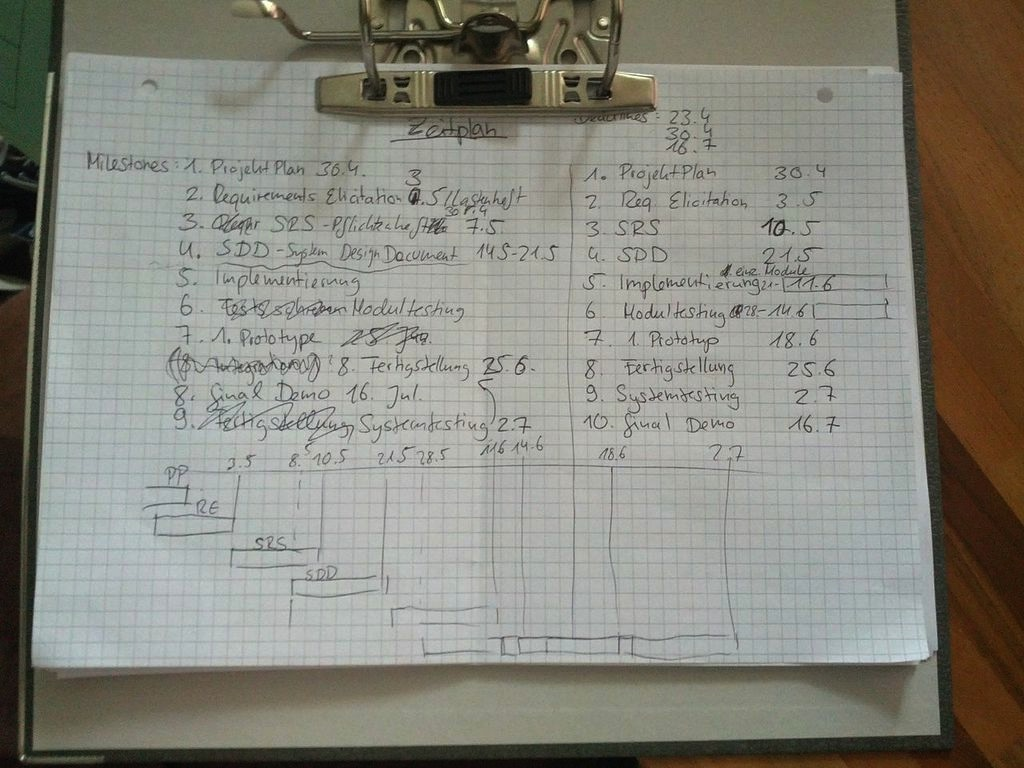
\includegraphics[scale=0.5]{Milestones.jpeg}
\\ \emph{Sieht wenig aus, doch ist wohl durchdacht}
\section{The project plan}
Nach Section 1.4 in der Aufgabenstellung (swp.pdf) den Projektplan anfertigen (bitte noch nicht einreichen) \\
\emph{Wird in einer kleinen Gruppe erledigt (Matthias Miller, Philipp Hilpert, Leonard Krämer}
\emph{
\section{Anmerkung}
Das Meeting war zu lang und etwas chaotisch, da 6 Leute an einem Tisch irgendwann unruhig werden.
}
\end{document}
